% !TeX root = ../main.tex
% Add the above to each chapter to make compiling the PDF easier in some editors.

\chapter{Groups}\label{cha:groups}
\section{Groups and Homomorphisms}
\subsection{Groups}
\begin{defn}[Semigroup, Monoid, and Group]\leavevmode
\begin{defnlist}
    \item A set $G$ with a mapping $\cdot$ on $G$ (that is, $\cdot: G \times G \to G$) is named \begin{itemize}
        \item \emph{semigroup}\index{semigroup} if $\forall a, b, c \in G.\ (a \cdot b) \cdot c = a \cdot (b \cdot c)$; \margintag{\emph{associativity}\index{associativity}}
        \item \mbox{\emph{monoid}\index{monoid} if it is a semigroup and $\exists e \in G.\ \forall a \in G.\ e \cdot a = a \cdot e = a$; \margintag{$e$ is called \emph{neutral element}\index{neutral element}}}
        \item \emph{group}\index{group} if it is a monoid and $\forall a \in G.\ \exists a' \in G.\ a \cdot a' = a' \cdot a = e$. \margintag{$a'$ is the \emph{inverse element}\index{inverse element} of $a$}
    \end{itemize}
    
    \item A group $(G,\cdot)$ is named \emph{abelian}\index{abelian group} or \emph{commutative}\index{commutativity} if the group operation $\cdot$ is commutative under elements of $G$, \begin{align}
        \forall a, b \in G.\quad a \cdot b = b \cdot a.
    \end{align}
    
    \begin{marginfigure}
        We denote groups by $(G,\cdot)$. If the group operation $\cdot$ is clear from context, we refer to the group simply as $G$. Subsequently, we also write $a b$ instead of $a \cdot b$.
    \end{marginfigure}
\end{defnlist}
\end{defn}

\begin{rmk}
Let $G$ be a group. Then, \begin{rmklist}
    \item there is exactly one neutral element $e \in G$ and for every $a \in G$ there is exactly one inverse element $a' \in G$, which we call $\inv{a}$;
    \item the mapping on $G$, which we refer to by $\cdot$, may be resembled by any symbol;
    \item if $G$ is abelian, often \begin{itemize}
        \item $+$ is used instead of $\cdot$,
        \item $0$ is used instead of $e$, and
        \item $-a$ is used instead of $\inv{a}$.
    \end{itemize}
\end{rmklist}
\end{rmk}

\begin{ex}{Semigroups, monoids, and groups}{}
\begin{center}
\setlength\tabcolsep{5pt}
\begin{tabular}{lrrrrr}
\toprule
 & $(\NO,+)$ & $(\NZ,+)$ & $(\Z,+)$ & $(\Z,\cdot)$ & $(\woZ{\Q},\cdot)$ \\
 \midrule
 semigroup & yes & yes & yes & yes & yes \\
 \addlinespace
 monoid & no & yes & yes & yes & yes \\
 \addlinespace
 group & yes & no & yes & no & yes \\
 \bottomrule
\end{tabular}
\end{center}
\end{ex}

\begin{ex}{General linear and special linear group}{}
The \emph{general linear group}\index{general linear group} $\GL{n}{K}$ is the group of invertible\marginfootnote{Recall from linear algebra that a matrix $\mA$ is invertible iff $\determ{\mA} \neq 0$.} ${n \times n}$ linear maps over a field\marginfootnote[1\baselineskip]{A \emph{field}\index{field} is a set of elements with well-defined operations for addition, subtraction, multiplication, and division. We give a formal definition in \cref{defn:field}. Examples of fields are the rational numbers $\Q$, the real numbers $\R$, and the complex numbers $\C$.} $K$, \begin{align}
    \GL{n}{K} \defeq \{\mA \in K^{n \times n} \mid \determ{\mA} \neq 0\}.
\end{align}

The \emph{special linear group}\index{special linear group} $\SL{n}{K}$ is the group of normed linear maps over the field $K$, \begin{align}
    \SL{n}{K} \defeq \{\mA \in K^{n \times n} \mid \determ{\mA} = 1\}.
\end{align}

The group operation of $\GL{n}{K}$ and $\SL{n}{K}$ is matrix multiplication. Their neutral element is the identity matrix $\mI$, and the inverse elements are the matrix inverses $\inv{\mA}$.
\end{ex}

\begin{ex}{Abelian groups}{}
\begin{itemize}
    \item $(\Z,+)$
    \item $(\Q,+)$
    \item $(\R,+)$
    \item $(\woZ{\R},\cdot)$
\end{itemize}
\end{ex}

\begin{ex}{Symmetric group}{}
The \emph{symmetric group}\index{symmetric group} $S_n$ is the group of bijections on the set $[n]$, \begin{align}
    S_n \defeq \{\sigma : [n] \to [n] \mid \text{$\sigma$ is bijective}\},
\end{align} with the function composition ``$\circ$'' as mapping.

Elements of the symmetric group ${\sigma \in S_n}$ are called \emph{permutations}\index{permutation}. The neutral element of the symmetric group is the identity $\id$, which maps each input to itself.

There are multiple ways of representing permutations. Perhaps the most natural representation of ${\sigma \in S_n}$ is a mapping in \emph{two-line notation}\index{two-line notation}, \begin{align}
    \sigma = \begin{pmatrix}
        1 & 2 & \cdots & n \\
        \sigma(1) & \sigma(2) & \cdots & \sigma(n) \\
    \end{pmatrix},
\end{align} or in \emph{one-line notation}\index{one-line notation} by simply omitting the first line, \begin{align}
    \sigma = (\sigma(1)\ \sigma(2)\ \cdots\ \sigma(n)).
\end{align}

An alternative characterization of a permutation is as a product of (disjoint) cycles. A \emph{cycle}\index{cycle} ${\rho \in S_n}$ is a permutation that maps a subset of numbers ${\{i_1, i_2, \dots, i_r\} \subseteq [n]}$ in a cyclic fashion. That is, \begin{align}
    \rho(i_1) = i_2,\quad \rho(i_2) = i_3,\quad \cdots\quad \rho(i_{r-1}) = i_r,\quad \rho(i_r) = i_1,
\end{align} leaving all other ${j \in [n]}$ fixed. We denote such a cycle by \begin{align}
    \rho = (i_1\ i_2\ \cdots\ i_r).
\end{align} A cycle of length $r$, is also called \emph{$r$-cycle}. 2-cycles are called \emph{transpositions}\index{transposition}.

Every permutation ${\sigma \in S_n}$ can be written as a ``product'' (i.e., composition), \begin{align}
    \sigma = \rho_1 \cdots \rho_s,
\end{align} where $\rho_i$ are cycles with pairwise disjunct elements. This is also known as the \emph{cycle notation}\index{cycle notation} of $\sigma$. Note that the ordering of $\rho_1, \dots \rho_s$ does not matter, as their elements are disjoint.

The cycle lengths $r_1, \dots, r_s$ (in descending order) of $\rho_1, \dots, \rho_s$ are the \emph{cycle type}\index{cycle type} of $\sigma$.

\begin{rmk}
The symmetric group is not abelian.
\end{rmk}\vspace{-20pt}\begin{proof}
We have $(1\ 2)(2\ 3) = (2\ 3\ 1)$ and $(2\ 3)(1\ 2) = (1\ 3\ 2)$.
\end{proof}
\end{ex}

\begin{lem}[Notation and Rules]
Let $(G,\cdot)$ be a group. \begin{lemlist}
    \item For $a \in G, n \in \NZ$, we write \begin{itemize}
        \item $a^n \defeq \underbrace{a \cdot a \cdots a}_{\text{$n$ many}}$,
        \item $a^0 \defeq e$, and
        \item $a^{-n} \defeq \underbrace{\inv{a} \cdot \inv{a} \cdots \inv{a}}_{\text{$n$ many}}$.
    \end{itemize}
    
    \item $\forall a, b \in G.\ \forall m, n \in \Z.$ \begin{nestedlemlist}
        \item $\inv{(\inv{a})} = a$
        \item $a^m \cdot a^n = a^{m+n}$, $(a^m)^n = a^{m \cdot n}$
        \item $\inv{(a \cdot b)} = \inv{b} \cdot \inv{a}$
    \end{nestedlemlist}
\end{lemlist}
\end{lem}
\begin{proof}[Proof of (b)(iii)] $(a \cdot b) \cdot \inv{b} \cdot \inv{a} = a \cdot \underbrace{(b \cdot \inv{b})}_{=e} \cdot \inv{a} = a \cdot \inv{a} = e$.
\end{proof}

\begin{defn}[Subgroup]
A subset $U \subseteq G$ is called a \emph{subgroup}\index{subgroup} of a group $G$ (denoted $U \leq G$) if $U$ itself is a group with mapping $\cdot$. That is, $U$ is a subgroup iff \begin{defnlist}
    \item $e \in U$; \margintag{$U$ contains the neutral element}
    \item $\forall a, b \in U.\quad a \cdot b \in U$; and \margintag{the mapping $\cdot$ is closed wrt. $U$}
    \item $\forall a \in U.\quad \inv{a} \in U.$ \margintag{the mapping $\inv{(\dots)}$ is closed wrt. $U$}
\end{defnlist} Associativity follows from $G$ being a group.
\end{defn}

\begin{ex}{Subgroups}{}
\begin{itemize}
    \item $\{e\}, G \leq G$ (\emph{trivial subgroups}\index{trivial subgroups})
    \item $\SL{n}{K} \leq \GL{n}{K}$
    \item Let $2\Z \defeq \{2m \mid m \in \Z\}$, then $(2\Z,+) \leq (\Z,+)$
\end{itemize}
\end{ex}

\begin{rmk}\label{rmk:cap_subgroup}
If $\{U_i\}_{i \in I}$ are subgroups of $G$, then $\bigcap_{i \in I} U_i \leq G$.
\end{rmk}

\begin{defn}[Generated Subgroup]
For any $M \subseteq G$, \begin{align}
    \gen{M} \defeq \bigcap_{\substack{U \leq G \\ M \subseteq U}} U \leq G, \margintag{by \cref{rmk:cap_subgroup}}
\end{align} is the \emph{subgroup generated by $M$}\index{generated subgroup}. In particular, $\gen{M}$ is the ``smallest'' subgroup that includes $M$.
\end{defn}

\begin{lem}
For $M \neq \emptyset$, we have \begin{align}
    \gen{M} = \{a_1 \cdot a_2 \cdots a_n \mid n \in \N, \text{$a_i \in M$ or $\inv{a_i} \in M$}\}.
\end{align}
\end{lem} \begin{proof}[Proof (sketch)]\leavevmode
Let $N \defeq \{a_1 \cdot a_2 \cdots a_n \mid n \in \N, \text{$a_i \in M$ or $\inv{a_i} \in M$}\}$.
\begin{itemize}
    \item \underline{$\gen{M} \subseteq N$}: $N \leq G$ and $M \subseteq N \implies \gen{M} \subseteq N$ \margintag{using that $\gen{M}$ is the smallest subgroup including $M$}
    \item \underline{$N \subseteq \gen{M}$}: if $U \leq G$ with $M \subseteq U$, then $U$ includes all of these products $\implies N \subseteq U \implies N \subseteq \gen{M}$ \qedhere
\end{itemize}
\end{proof}

\begin{ex}{Generated subgroup}{}
$S_3 = \{\id, \underbrace{(1\ 2)}_{\tau_1}, \underbrace{(1\ 3)}_{\tau_2}, \underbrace{(2\ 3)}_{\tau_3}, \underbrace{(1\ 2\ 3)}_{\sigma_1}, \underbrace{(1\ 3\ 2)}_{\sigma_2}\} = \gen{\{\underbrace{(1\ 2)}_{\tau_1}, \underbrace{(1\ 2\ 3)}_{\sigma_1}\}}$.
\end{ex}

\begin{defn}[Cyclic Group]
A group $G$ is \emph{cyclic}\index{cyclic group} if $\exists a \in G$ with \begin{align}
    G = \gen{a} \defeq \gen{\{a\}} = \{a^m \mid m \in \Z\}.
\end{align} Such an $a \in G$, is called a \emph{generator}\index{generator} of $G$.
\end{defn}

\begin{marginfigure}
    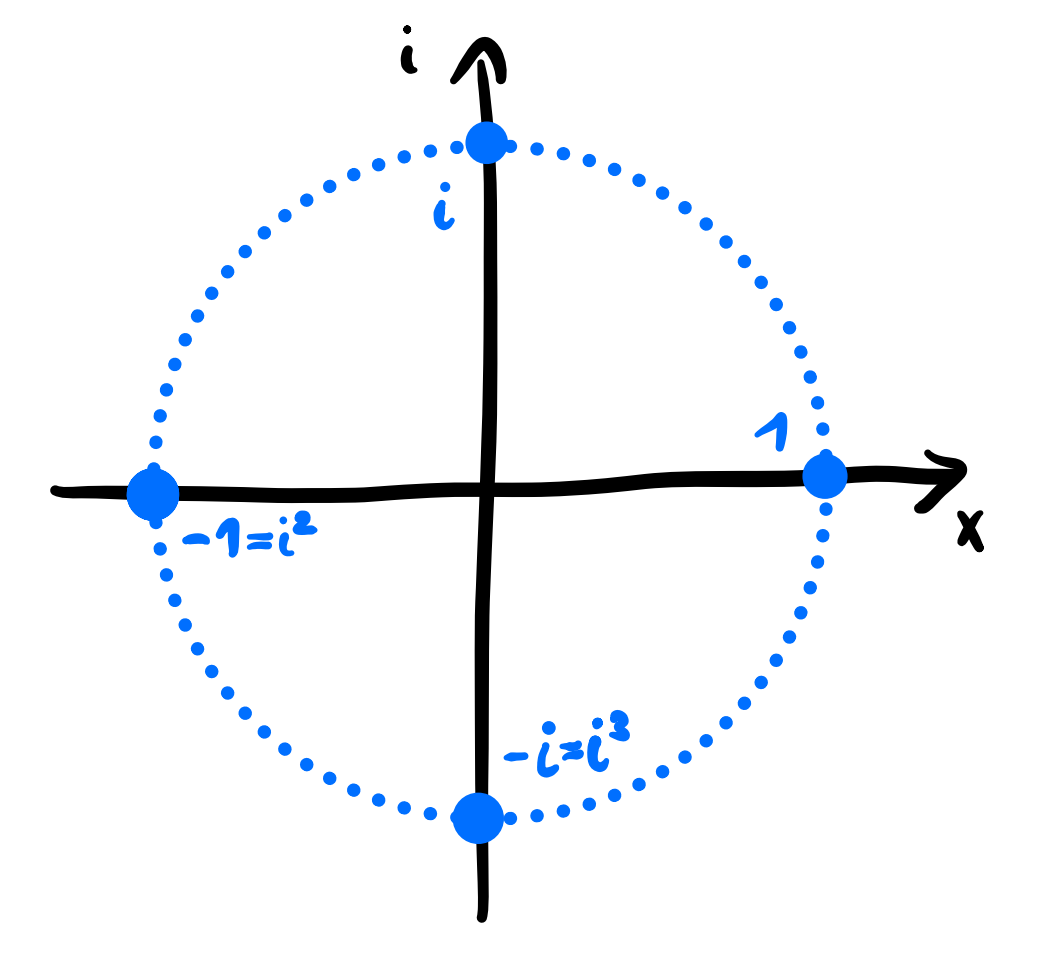
\includegraphics[width=\textwidth]{c_cyclic_subgroup.png}
    \caption{An illustration of the cyclic subgroup $\gen{i}$ in the complex plane.}
\end{marginfigure}

\begin{ex}{Cyclic groups}{}
\begin{itemize}
    \item $\gen{i} = \{i^m \mid m \in \Z\}$ is a cyclic subgroup of $(\woZ{\C},\cdot)$, \begin{align*}
        \gen{i} &= \{\dots, \underbrace{i^{-2}}_{=-1}, \underbrace{i^{-1}}_{=-i}, 1, i, \underbrace{i^2}_{=-1}, \underbrace{i^3}_{=-i}, \underbrace{i^4}_{=1}, \underbrace{i^5}_{=i}, \dots\} \\
                &= \{1, i, -1, -i\}.
    \end{align*}
    \item $(\Z,+) = \gen{1} = \{\dots, -2, -1, 0, 1, 2, \dots\}$ is cyclic
\end{itemize}
\end{ex}

\begin{defn}[Order]\index{order}
Let $G$ be a group.
\begin{defnlist}
    \item The cardinality $|G| \in \wInfty{\N}$ is called \emph{order} of the group $G$.
    \item For any $a \in G$, $o(a) \defeq |\gen{a}|$ is the \emph{order} of the element $a$.
\end{defnlist} If $|G| < \infty$, $G$ is called \emph{finite}\index{finite group}.
\end{defn}

\begin{lem}
If $k \defeq o(a) < \infty$, we have \begin{lemlist}
    \item $o(a) = \min\{j \in \N \mid a^j = e\}$;
    \item $\gen{a} = \{e, a, a^2, \dots, a^{k-1}\}$; and
    \item\label{lem:order_identity} For any $j \in \Z$, $a^j = e \iff \divides{o(a)}{j}$.\footnote{We use $\divides{a}{b}$ to denote that $a$ divides $b$.}
\end{lemlist}
\end{lem} \begin{proof}
We write $m \defeq \min\{j \in \N \mid a^j = e\}$. \begin{itemize}
    \item \underline{$\{e, a, a^2, \dots, a^{m-1}\} \subseteq \gen{a}$}: Let us fix an arbitrary $j \in \N$. We have, \begin{align*}
        o(a) = |\gen{a}| < \infty &\implies \exists j' > j.\ a^j = a^{j'} \margintag{as the order of $a$ is finite} \\
                                  &\implies a^{j'-j} = e \margintag{by multiplying from the right with $a^{-j}$} \\
                                  &\implies \text{$m$ exists and $\{e, a, a^2, \dots, a^{m-1}\} \subseteq \gen{a}$}. \margintag{as $j'-j \in \N$ is again a natural number}
    \end{align*}
    \item \underline{$\gen{a} \subseteq \{e, a, a^2, \dots, a^{m-1}\}$}: We fix any $n \in \Z$. Then, by \emph{long division}\index{long division}, there exist $q, r \in \Z$ and $0 \leq r < m$ with $n = q \cdot m + r$. This yields, \begin{align*}
        a^n = a^{q \cdot m + r} = \underbrace{(a^m)^q}_{=e} \cdot a^r = a^r \in \{e, a, a^2, \dots, a^{m-1}\}.
    \end{align*}
\end{itemize} This proves that $m = o(a)$ and $\gen{a} = \{e, a, a^2, \dots, a^{m-1}\}$. It also follows that \begin{align*}
    a^n = e \iff r = 0 \iff \divides{m}{n}. &\qedhere
\end{align*}
\end{proof}

\begin{rmk}
For a finite cyclic group $\gen{a} = \{e, a, a^2, \dots, a^{k-1}\}$ of order $k$, we have $a^{k-j} = a^{-j}$.
\end{rmk}

\begin{ex}{Order}{order}
\begin{itemize}
    \item Let us consider $\GL{2}{\R}$. Then, \begin{align*}
        \mA = \begin{bmatrix}
            2 & 0 \\
            0 & 2 \\
        \end{bmatrix} &\implies \forall n \in N.\ \mA^n = \begin{bmatrix}
            2^n & 0 \\
            0 & 2^n \\
        \end{bmatrix} \neq \mI \\ &\implies o(\mA) = \infty, \\
        \mB = \begin{bmatrix}
            0 & 1 \\
            -1 & 0 \\
        \end{bmatrix} &\implies \begin{multlined}[t]\mB^2 = \begin{bmatrix}
            -1 & 0 \\
            0 & -1 \\
        \end{bmatrix}, \\ \mB^3 = -\mB = \begin{bmatrix}
            0 & -1 \\
            1 & 0 \\
        \end{bmatrix}, \mB^4 = (\mB^2)^2 = \mI\end{multlined} \\ &\implies o(\mB) = 4.
    \end{align*}
    
    \item $o(S_n) = |S_n| = |\{\sigma : [n] \to [n] \mid \text{$\sigma$ is bijective}\}| = n!$
    
    \item Let us find the subgroups of \begin{align*}
        S_3 = \{\id, (1\ 2), (1\ 3), (2\ 3), (1\ 2\ 3), (1\ 3\ 2)\}.
    \end{align*} We immediately obtain the trivial subgroups $\{\id\}$ and $S_3$ or order $1$ and $6$, respectively. It is a simple exercise to confirm the following cyclic subgroups: \begin{itemize}
        \item $\gen{(1\ 2)} = \{\id, (1\ 2)\}$
        \item $\gen{(1\ 3)} = \{\id, (1\ 3)\}$
        \item $\gen{(2\ 3)} = \{\id, (2\ 3)\}$
        \item $\gen{(1\ 2\ 3)} = \gen{(1\ 3\ 2)} = \{\id, (1\ 2\ 3), (1\ 3\ 2)\}$
    \end{itemize} The first three subgroups generated by 2-cycles are of order 2, the last subgroup generated by the 3-cycles is of order 3.
    
    Observe that the subgroup orders are divisors of the group order. This is not coincidental, we will make this precise in the following. In doing so, we will also find that our list of subgroups of $S_3$ was indeed exhaustive.
\end{itemize}
\end{ex}

\begin{marginfigure}
    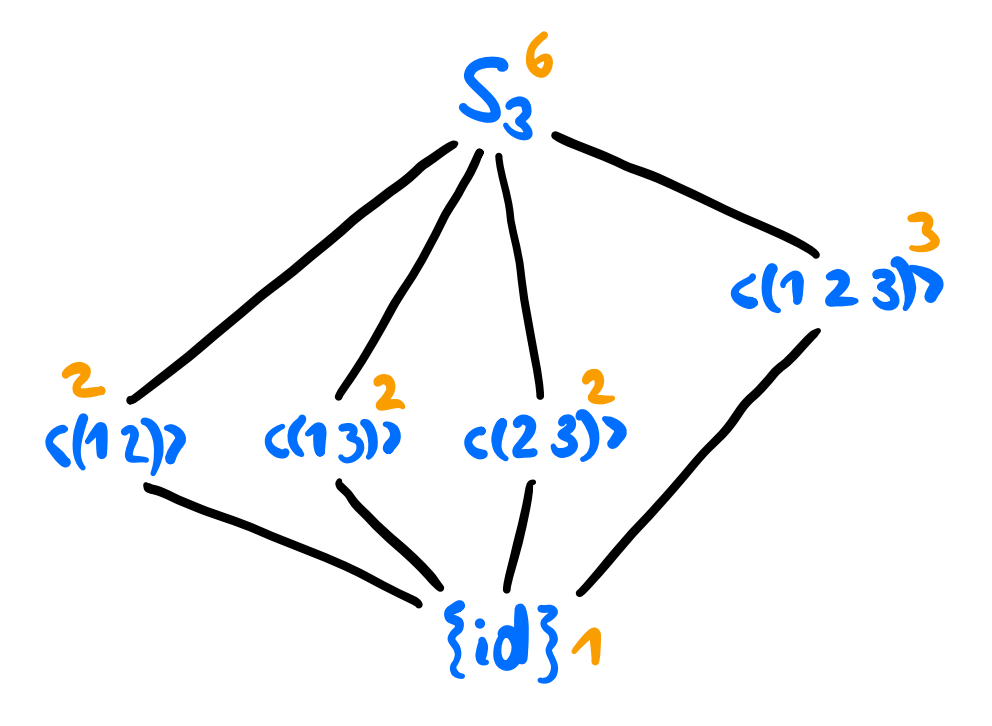
\includegraphics[width=\textwidth]{s3_subgroup_graph.png}
    \caption{Subgroup graph of the symmetric group $S_3$.}\label{fig:s3_subgroup_graph}
\end{marginfigure}
    
The subgroup structure of a group $G$ can be graphically represented in a \emph{subgroup graph}\index{subgroup graph}. Subgroups of $G$ are represented as vertices. Groups $U$ and $V$ are connected if $U \leq V$ and there exists no subgroup ``between'' $U$ and $V$. An example is given in \cref{fig:s3_subgroup_graph}.

\begin{defn}[Cosets and Index]
Let $U \leq G$ be a subgroup.
\begin{defnlist}
    \item For $a \in G$, \begin{align}
        aU &\defeq \{a \cdot u \mid u \in U\}, \\
        Ua &\defeq \{u \cdot a \mid u \in U\},
    \end{align} are the left\index{left coset} and right\index{right coset} \emph{coset}\index{coset} of $U$ in $G$, respectively.
    \item The \emph{index}\index{index} $[G : U] \defeq |\{aU \mid a \in G\}|$ of $U$ in $G$ is defined as the number of cosets of $U$ in $G$.\footnote{The number of left cosets is identical to the number of right cosets.}
\end{defnlist}
\end{defn}

\begin{lem}
For all $a, b \in G$, we have
\begin{lemlist}
    \item $aU = U \iff a \in U$
    \item $aU = bU \iff \inv{a} b \in U$
    \item $aU \cap bU \neq \emptyset \iff aU = bU$
    \item $G = \bigcup_{a \in G} aU$
    \item\label{lem:cosets_size} $|aU| = |U|$
\end{lemlist}
\end{lem} \begin{proof}[Proof of (v)]
$U \to aU, u \mapsto a \cdot u$ is a bijective mapping. Hence, domain and codomain are of the same size.
\end{proof}

\begin{thm}[Lagrange's Theorem]\index{Lagrange's theorem}\label{thm:lagrange}
If $G$ is a finite group and $U \leq G$ is some subgroup, then \begin{align}
    |G| = |U| \cdot [G : U].
\end{align} In particular, $|U|$ and $[G : U]$ are divisors of $|G|$.
\end{thm} \begin{proof}
Let $r \defeq [G:U]$. Then we can write $G$ as a disjoint union of cosets, \begin{align*}
    G = a_1 U \cupdot a_2 U \cupdot \cdots \cupdot a_r U.
\end{align*} We have, \begin{align*}
    |G| = \sum_{i=1}^r |a_i U| = r \cdot |U| = [G:U] \cdot |U|. \margintag{using that $|a_i U| = |U|$ by \cref{lem:cosets_size}} &\qedhere
\end{align*}
\end{proof}

\begin{cor}
Let $G$ be a finite group. Then we have for any $a \in G$, \begin{corlist}
    \item $\divides{o(a)}{|G|}$
    \item $a^{|G|} = e$ \quad (\emph{Fermat's little theorem}\index{Fermat's little theorem})
\end{corlist}
\end{cor} \begin{proof}
\leavevmode\begin{corlist}
\item By \hyperref[thm:lagrange]{Lagrange's theorem}, $\divides{|\gen{a}|}{|G|}$.
\item By \cref{lem:order_identity}, $a^{|G|} = e \iff \divides{o(a)}{|G|}$. \qedhere
\end{corlist}
\end{proof}

\begin{cor}\label{cor:prime_group_is_cyclic}
Let $G$ be a group such that $|G| = p$ where $p$ is prime. Then, $G$ is cyclic.
\end{cor} \begin{proof}
\begin{align*}
    |G| > 1 &\implies \exists a \in G \setminus \{e\} \\
            &\implies \divides{1 \neq |\gen{a}|}{|G|} \margintag{using that $o(a) \geq 2$ if $a \neq e$ and \hyperref[thm:lagrange]{Lagrange's theorem}} \\[5pt]
            &\implies |\gen{a}| = p = |G|. \margintag{using that $|G|$ only has divisors $1$ and $p$}
\end{align*} Therefore, $\gen{a} = G$.
\end{proof}

\begin{ex}{Subgroups of $S_3$}{}
We will now see that $S_3$ has exactly four non-trivial subgroups, proving that we have found all subgroups of $S_3$ in \cref{ex:order}.

Let ${U \leq S_3}$ be a non-trivial subgroup. By \hyperref[thm:lagrange]{Lagrange's theorem}, we have ${\divides{|U|}{|S_3| = 3! = 6}}$. As we have excluded the trivial subgroups $\{\id\}$ and $S_3$, we know that ${|U| \neq 1, 6}$. This leaves us with ${|U| \in \{2,3\}}$.

Observe that $2$ and $3$ are prime, hence, by \cref{cor:prime_group_is_cyclic} $U$ must be cyclic. Recall that we have already enumerated all (four) cyclic subgroups of $S_3$ in \cref{ex:order}.
\end{ex}

\subsection{Homomorphisms}

\section{Normal Subgroups and Quotient Groups}
\section{Homomorphism and Isomorphism Theorems}
\section{Group Actions}
\section{Sylow Theorems}
\section{Direct products and Abelian Groups}
\section{Solvable Groups}
